% Draft for the 5-minute pitch; the final version goes to Google Slides.
\documentclass[aspectratio=169,11pt]{beamer}
\usetheme{default}
\usecolortheme{seahorse}
\setbeamertemplate{navigation symbols}{}
\setbeamertemplate{footline}[frame number]
\usepackage{booktabs}

\title{Hesai AT512 for Emergency Brake Assist}
\subtitle{Lidar performance -- statistical modelling (Exercise 3)}
\author{Team: \textit{names TBD}}
\date{3DSSF -- Kozma}

\begin{document}

\begin{frame}
  \titlepage
\end{frame}

% ---------------------------------------------------------------
\begin{frame}{The lidar: Hesai AT512}
  \begin{columns}[T]
    \column{0.56\textwidth}
    \small
    \begin{tabular}{ll}
      \toprule
      range          & 300\,m @ 10\,\% refl.\ (400\,m max) \\
      resolution     & 0.05$^\circ$ $\times$ 0.05$^\circ$ \\
      field of view  & 120$^\circ$ $\times$ 25.6$^\circ$ \\
      points         & 12.3\,M/s = 2400 $\times$ 512 @ 10\,Hz \\
      \bottomrule
    \end{tabular}
    \column{0.4\textwidth}
    \textbf{Why this one}
    \begin{itemize}
      \item automotive-grade, long-range series product
      \item very fine angular grid $\rightarrow$ many beams on small, far objects
      \item 120$^\circ$ covers adjacent lanes
    \end{itemize}
  \end{columns}
  \vspace{1em}
  \small\textit{Assumption: the 300\,m spec means 90\,\% detection probability (not stated by Hesai).}
\end{frame}

% ---------------------------------------------------------------
\begin{frame}{Model: returns per frame are a random variable}
  \begin{columns}[T]
    \column{0.5\textwidth}
    \textbf{1. Beams on target} (W $\times$ H object at $R$)
    \[
      n = \frac{W}{R\,\Delta\theta_h}\cdot\frac{H}{R\,\Delta\theta_v}
    \]
    random grid offset $\rightarrow$ $n$ rounds up or down

    \vspace{0.5em}
    \textbf{2. Each beam returns with probability} (echo $\propto \rho/R^2$)
    \[
      p = 1 - e^{-C\rho/R^2}, \quad p(300\,\text{m}, 10\,\%) = 0.9
    \]

    \vspace{0.2em}
    \textbf{3. Returns:} $K \sim \mathrm{Binomial}(n, p)$\\
    \textbf{Requirement:} $P(K \ge 5) \ge 99\,\%$ at 250\,m
    \column{0.46\textwidth}
    \textbf{Example:} pedestrian, 10\,\%, 350\,m\\[0.3em]
    \small
    \begin{tabular}{lcccccccccc}
      \toprule
      frame   & 1 & 2 & 3 & 4 & 5 & 6 & 7 & 8 \\
      beams   & 12 & 12 & 12 & 6 & 6 & 12 & 6 & 6 \\
      returns & 11 & 10 & 10 & 5 & 5 & 10 & \textcolor{red!70!black}{\textbf{4}} & \textcolor{red!70!black}{\textbf{3}} \\
      \bottomrule
    \end{tabular}

    \vspace{0.8em}
    \normalsize
    average $E[K] = 7.9 \ge 5$\\
    but $P(K < 5) = 12\,\%$ $\rightarrow$ \textbf{fails}

    \vspace{0.5em}
    \small\textit{The average can pass while the probability fails.}
  \end{columns}
\end{frame}

% ---------------------------------------------------------------
\begin{frame}{Results (10\,\% reflectivity)}
  \centering
  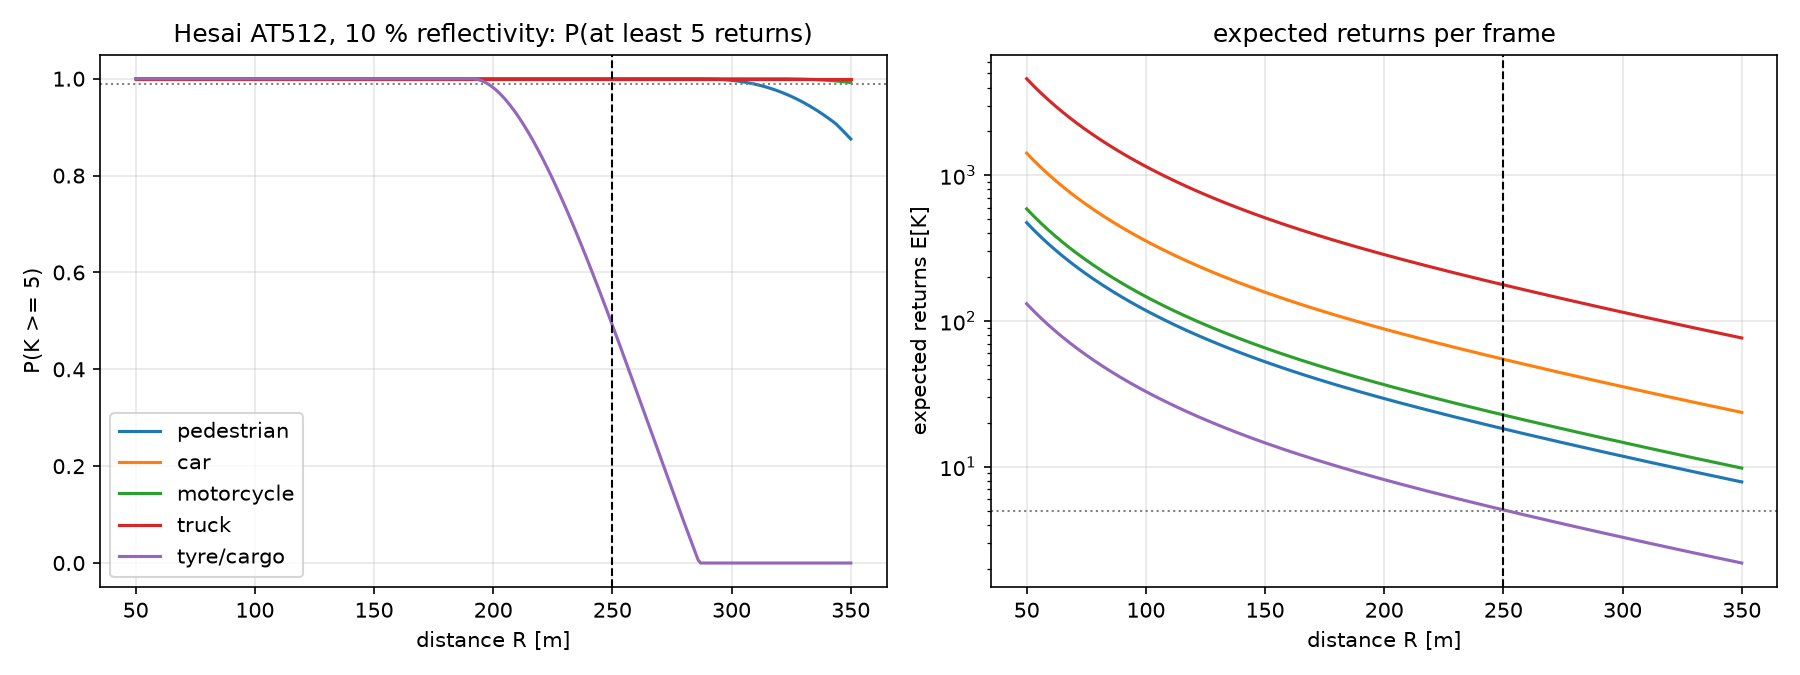
\includegraphics[width=0.95\textwidth]{lidar_eba.png}\\[0.3em]
  \small
  $P(K \ge 5)$ at 250\,m: pedestrian and all vehicles $> 99.99\,\%$, \quad
  tyre (0.5\,m) \textcolor{red!70!black}{\textbf{49\,\%}}
\end{frame}

% ---------------------------------------------------------------
\begin{frame}{Conclusion}
  \begin{columns}[T]
    \column{0.5\textwidth}
    \textbf{AT512 fulfils EBA}
    \begin{itemize}
      \item all vehicles and pedestrians at 250\,m, even at 10\,\% reflectivity
      \item 99\,\% range: pedestrian 308\,m, motorcycle 353\,m, car/truck $\ge$ 400\,m
      \item small debris ($\sim$0.5\,m): only up to $\approx$ 200\,m -- too few beams hit (resolution limit, not reflectivity)
    \end{itemize}
    \column{0.46\textwidth}
    \textbf{Limitations}
    \begin{itemize}\small
      \item flat, frontal targets
      \item independent beams -- optimistic in rain / dirty sensor
      \item 90\,\% behind the 300\,m spec is assumed
      \item single frame; at 130\,km/h, 34 frames remain before braking must start
    \end{itemize}
  \end{columns}
\end{frame}

\end{document}
